The scintillation yield provided by the manufacturer, $8000~\text{photons}/\MeV$, is only valid for minimum ionizing particles (MIP). As tritium electron energies are not MIP particles, the output light generated by the scintillating fibres was studied. The emission of scintillation photons were also simulated.

When particles that are not MIP are detected in plastic scintillators, an output light quenching effect happens, which can be parametrized by the Birk's coefficient\cite{BirksPaper}, 
\begin{equation}
\frac{dL}{dx}= S\frac{\displaystyle{\frac{dE}{dx}}}{1+k_B\displaystyle{\frac{dE}{dx}}}
\label{eq:birkscoefficient}
\end{equation}
Where $\frac{dL}{dx}$ is the output light per unit of path length, $\frac{dE}{dx}$ is the energy deposited per unit of path length and S is the scintillation yield for MIPs, provided by the manufacturer. A Birk's coefficient $k_B=0.126~\mm/\MeV$ is typically used for scintillators based on polystyrene \cite{BirksCoefficient}. In this section, the importance of this quenching effect and how it affects the tritium detection is discussed.

A study of the energy deposition of tritium electrons on scintillating fibres was carried out. In Figure \ref{fig:InitialFinalTritiumEnergy} the initial energy of simulated tritium electrons that reach the scintillating fibres is compared to the energy deposited in them. A shift to lower energies is observed, caused by the energy loss of tritium electrons in water is observed. The cut at about $1~\keV$ visible in both energy distributions is produced by the default energy threshold of $990~\eV$ in the G4EmLivermorePhysics list.
\begin{figure}[h]
\centering
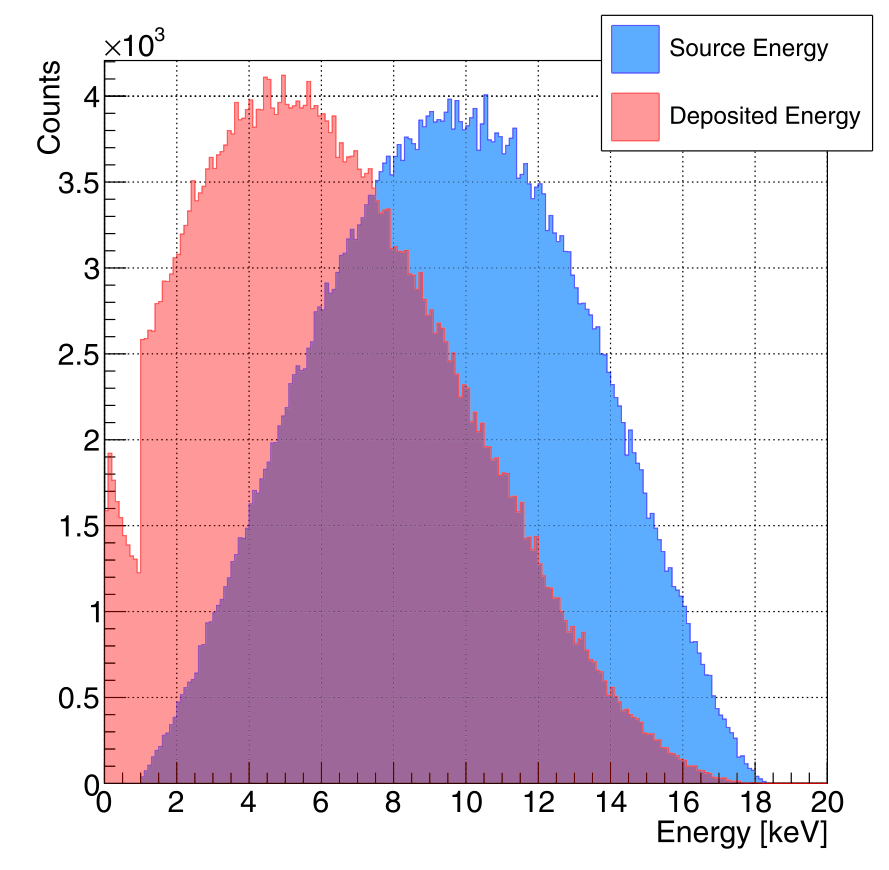
\includegraphics[scale=0.3]{6Simulations/61TRITIUMDesign/612Outputlight/InitialandFinalTritiumEnergy.png}
\caption{Distribution of the initial energy of tritium events that reach the scintillating fibres (blue histogram) and the energy deposited in them (red histogram) \cite{SimulationPaperCarlos}.\label{fig:InitialFinalTritiumEnergy}}
\end{figure}
Figure \ref{fig:BirksEffectinEnergyDistribution} shows two distributions of the number of photons produced in scintillating fibres by tritium events, one in which the quenching effect is not considered ($k_B=0$) and the other with the Birk's coefficient set to $k_B=0.126~\mm/\MeV$.
\begin{figure}[h]
\centering
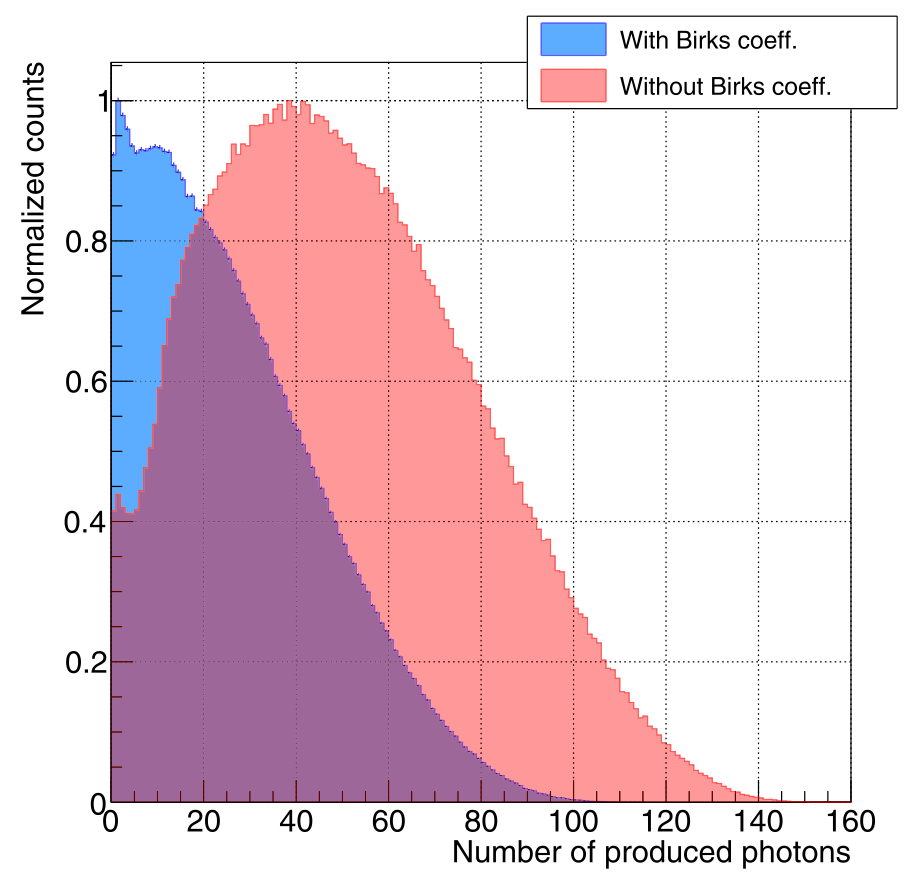
\includegraphics[scale=0.3]{6Simulations/61TRITIUMDesign/612Outputlight/BirksEnergyDistribution.png}
\caption{Energy distributions of photons produced in the scintillating fibre, without the Birk's coefficient (red histogram) and with the Birk's coefficient $k_B=0.126~\mm/\MeV$ (blue histogram)\cite{SimulationPaperCarlos}.\label{fig:BirksEffectinEnergyDistribution}}
\end{figure}  
A distribution with a peak close to 40 photons per tritium event and a maximum near 150 photons were obtained when the quenching effect is not considered. A significant reduction of the output light is observed when the Birk's coefficient is included, obtaining a distribution peaked at around $10$ photons and a maximum of $110$ photons. The quenching effect is also observed in Figure \ref{fig:2DimPlotBirks}, in which the number of photons produced  as a function of the energy deposited in the fibres is displayed in a two-dimensional plot. In this figure, in addition to a reduction of the number of photons produced per unit of energy deposited, a broader distribution is obtained when the Birk's coefficient is considered, indicating an increase of the fluctuations of the energy deposited.

\begin{figure}
\centering
    \begin{subfigure}[b]{0.4\textwidth}
    \centering
    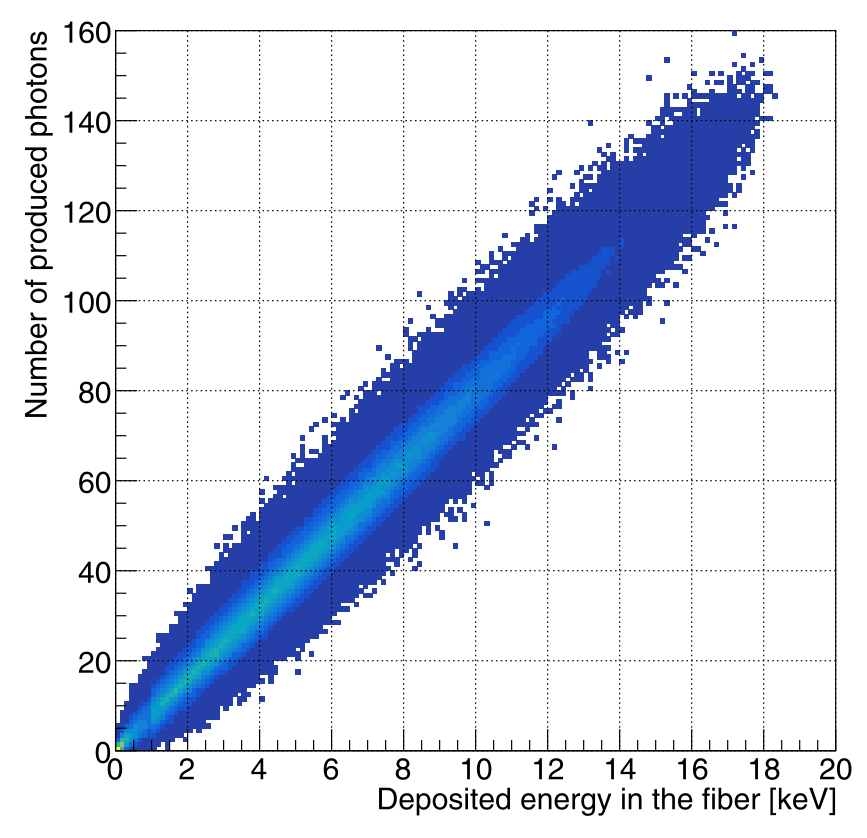
\includegraphics[width=\textwidth]{6Simulations/61TRITIUMDesign/612Outputlight/BidimensionalPlotBirksOFF.png}  
    \caption{\label{subfig:2DimPlotNoBirks}}
    \end{subfigure}
    \hfill
    \begin{subfigure}[b]{0.4\textwidth}
    \centering
    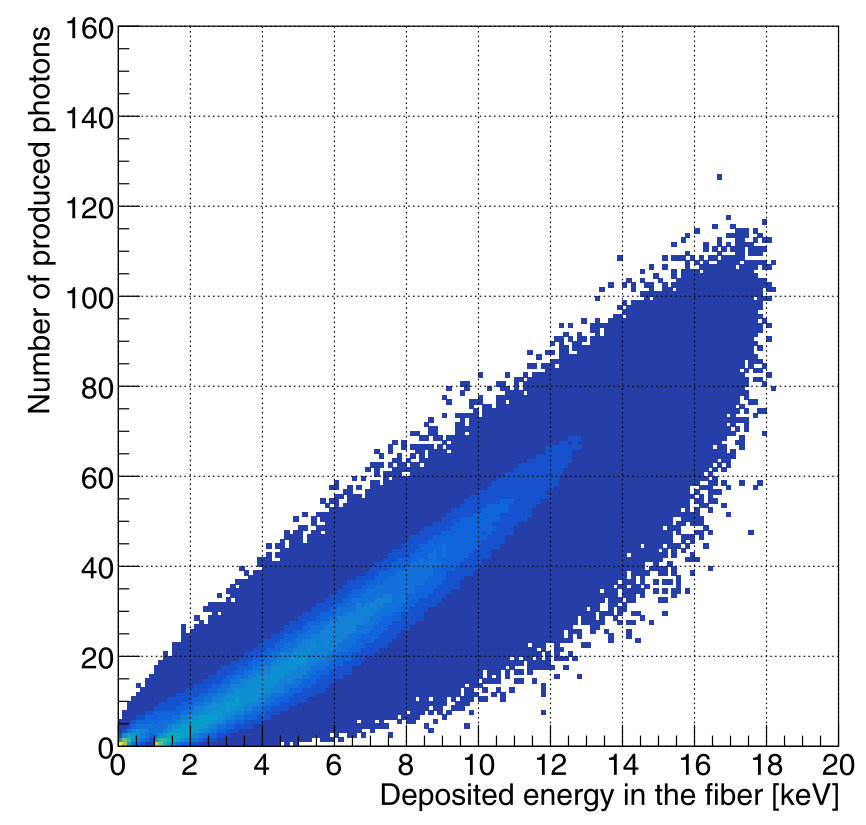
\includegraphics[width=\textwidth]{6Simulations/61TRITIUMDesign/612Outputlight/BidimensionalPlotBirksON.png}  
    \caption{\label{subfig:2DimPlotBirks}}
    \end{subfigure}
 \caption{Number of photons produced versus the energy deposited in the scintillating fibres when a) $k_B=0$ b) $k_B=0.126~\mm/\MeV$ \cite{SimulationPaperCarlos}.}
 \label{fig:2DimPlotBirks}
\end{figure}